\subsection{Le Menu}

	Le menu a 4 liens principaux : 
	\begin{description}
		\item[Acheter :] Renvoie vers les catégories de produits achetables.
		\item[Louer :] Renvoie vers les catégories de produits louables.
		\item[A Propos :] Affichage d'informations relatives à Brico-Bob.
		\item[Contact :] Affiche les coordonnées des administrateurs du site\\
		 ( et du service 	client par exemple ).
	\end{description}

	Le menu est aussi déroulant lorsque l'utilisateur survole "Acheter" et "Louer", 	ce qui lui permet d'accéder directement aux catégories de produits.
	
	\subsection{Catégories - Sous catégories}

	Une catégorie ou une sous catégorie peut contenir soit d'autre catégories, 	soit des produits. Il est donc techniquement avoir une arborescence comme ceci par exemple :

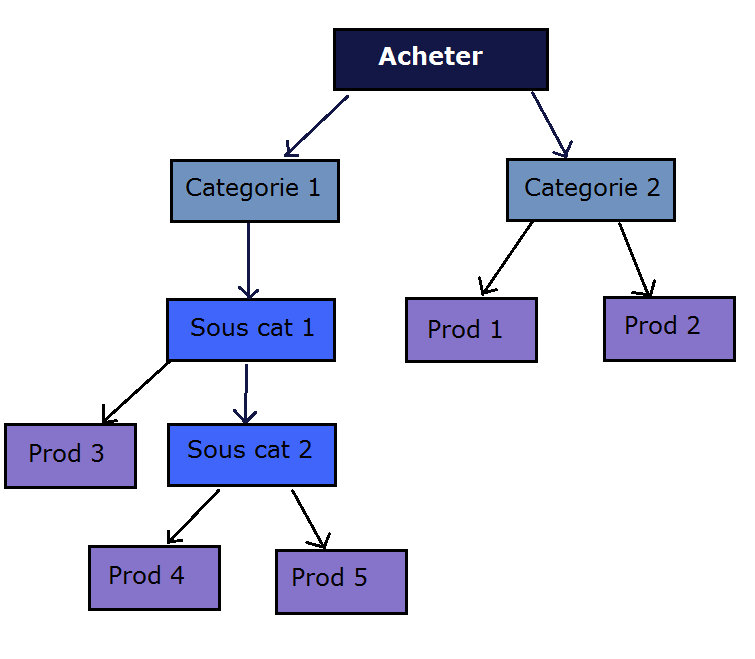
\includegraphics[scale=0.7]{arbocatego.png}

	\subsection{Fiche produit}

	La fiche produit contiens les informations relatives au produit, les liens pour l'acheter ou le louer, et les avis des utilisateurs.
Chaque utilisateur peut ajouter un commentaire et "noter le produit", un peu comme sur un blog. Le formulaire d'ajout d'un commentaire se trouve en
bas de la page fiche produit. 
		
	\subsection{Coups de cœur}

	Les coups de cœur sur la page d'accueil représentent des produits à mettre en valeur, qui sont par exemple le dernier produit ajouté dans la base de donnée afin d'en assurer sa promotion
		
	\subsection{Panneau d'administration}

	Lorsque l'administrateur se connecte, il a accès au panneau d'administration. Ce panneau lui permet plusieurs choses comme cela est expliqué :
	
	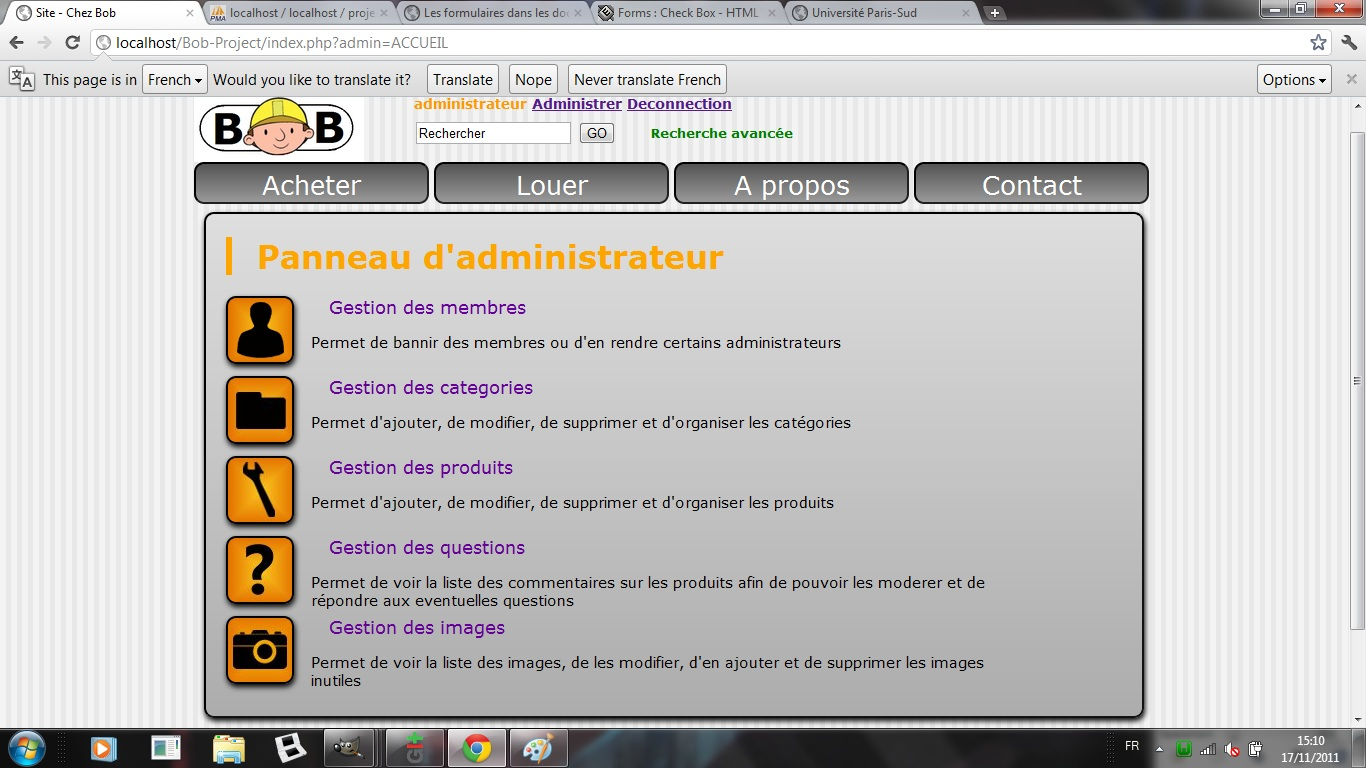
\includegraphics[scale=0.5]{panneauadmin.jpg}